% This file was created with tikzplotlib v0.10.1.
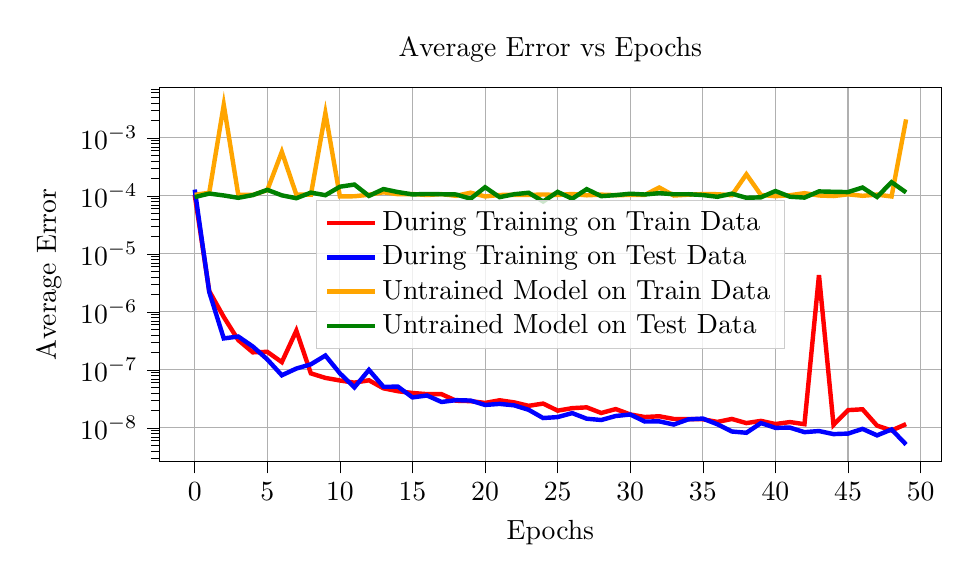
\begin{tikzpicture}

    \definecolor{darkgray176}{RGB}{176,176,176}
    \definecolor{green}{RGB}{0,128,0}
    \definecolor{lightgray204}{RGB}{204,204,204}
    \definecolor{orange}{RGB}{255,165,0}
    
    \begin{axis}[
      width = 0.95\textwidth,
      height = 18em,
    legend cell align={left},
    legend style={
      fill opacity=0.8,
      draw opacity=1,
      text opacity=1,
      at={(0.5,0.5)},
      anchor=center,
      draw=lightgray204
    },
    % log basis y={10},
    tick align=outside,
    tick pos=left,
    title={Average Error vs Epochs},
    x grid style={darkgray176},
    xlabel={Epochs},
    xmajorgrids,
    xmin=-2.45, xmax=51.45,
    xtick style={color=black},
    y grid style={darkgray176},
    ylabel={Average Error},
    ymajorgrids,
    ymin=2.63604330184737e-09, ymax=0.00725950156863836,
    ymode=log,
    ytick style={color=black},
    ytick={1e-10,1e-09,1e-08,1e-07,1e-06,1e-05,0.0001,0.001,0.01,0.1},
    yticklabels={
      \(\displaystyle {10^{-10}}\),
      \(\displaystyle {10^{-9}}\),
      \(\displaystyle {10^{-8}}\),
      \(\displaystyle {10^{-7}}\),
      \(\displaystyle {10^{-6}}\),
      \(\displaystyle {10^{-5}}\),
      \(\displaystyle {10^{-4}}\),
      \(\displaystyle {10^{-3}}\),
      \(\displaystyle {10^{-2}}\),
      \(\displaystyle {10^{-1}}\)
    }
    ]
    \addplot [ultra thick, red]
    table {%
    0 0.000104205340903718
    1 2.2795081804361e-06
    2 8.16013880466926e-07
    3 3.26127519656438e-07
    4 2.00797316551871e-07
    5 2.04524624791702e-07
    6 1.36023288632714e-07
    7 4.74071129019649e-07
    8 8.70571454925084e-08
    9 7.27430773395099e-08
    10 6.5652713487907e-08
    11 6.02018914719338e-08
    12 6.61969394855078e-08
    13 4.81310458155804e-08
    14 4.2873633532281e-08
    15 3.99703772302473e-08
    16 3.81714855279824e-08
    17 3.8142367486671e-08
    18 2.93974711240708e-08
    19 2.89232531258676e-08
    20 2.69239741612637e-08
    21 2.99225142441628e-08
    22 2.75352860512612e-08
    23 2.4009436216943e-08
    24 2.62635957426482e-08
    25 1.98318286237509e-08
    26 2.18844142807484e-08
    27 2.25979448487124e-08
    28 1.80841581709501e-08
    29 2.10961470514803e-08
    30 1.70547433953061e-08
    31 1.53920822754117e-08
    32 1.58656572324389e-08
    33 1.42510874212576e-08
    34 1.41820661880843e-08
    35 1.4081289023693e-08
    36 1.26731078964326e-08
    37 1.42557086135753e-08
    38 1.21001750841288e-08
    39 1.32015909315442e-08
    40 1.16595693100408e-08
    41 1.26017134505219e-08
    42 1.15926468424732e-08
    43 4.30966929343413e-06
    44 1.12703659738145e-08
    45 2.02334238252888e-08
    46 2.09316262100856e-08
    47 1.09466631315058e-08
    48 9.01701913136321e-09
    49 1.16273870531813e-08
    };
    \addlegendentry{During Training on Train Data}
    \addplot [ultra thick, blue]
    table {%
    0 0.000128205894725397
    1 2.19211028706923e-06
    2 3.48693362184349e-07
    3 3.7564521448985e-07
    4 2.53075398859437e-07
    5 1.51381684077023e-07
    6 8.07240780886787e-08
    7 1.05399159622266e-07
    8 1.24686110325456e-07
    9 1.76708667254388e-07
    10 8.71838210514397e-08
    11 4.9951530911585e-08
    12 9.98501263893559e-08
    13 5.1198544070985e-08
    14 5.13218765263446e-08
    15 3.35316165944732e-08
    16 3.61962158024198e-08
    17 2.79910761236124e-08
    18 3.00771283434642e-08
    19 2.95923321402825e-08
    20 2.4853880731257e-08
    21 2.59286903059319e-08
    22 2.44853541886414e-08
    23 2.05111181372786e-08
    24 1.47937218031302e-08
    25 1.5353929683215e-08
    26 1.79923898002698e-08
    27 1.44036702565131e-08
    28 1.36676279183234e-08
    29 1.603949861817e-08
    30 1.70154574874459e-08
    31 1.28716752811897e-08
    32 1.29476260823935e-08
    33 1.14277387552875e-08
    34 1.4037178530657e-08
    35 1.44796095113975e-08
    36 1.15444818149513e-08
    37 8.66101146357323e-09
    38 8.24099988250282e-09
    39 1.21144925202543e-08
    40 1.00226200672182e-08
    41 1.01044204114942e-08
    42 8.44652703335669e-09
    43 8.82723494299853e-09
    44 7.81588394005439e-09
    45 7.98052735007104e-09
    46 9.61182422543061e-09
    47 7.4352684009682e-09
    48 9.4029859454281e-09
    49 5.17222886742275e-09
    };
    \addlegendentry{During Training on Test Data}
    \addplot [ultra thick, orange]
    table {%
    0 0.000104004502645694
    1 0.000113090267404914
    2 0.00369982863776386
    3 0.000103595812106505
    4 0.000103680438769516
    5 0.000125327438581735
    6 0.000573276192881167
    7 0.000104799939435907
    8 0.000104467922938056
    9 0.00266967760398984
    10 9.74361173575744e-05
    11 9.83515856205486e-05
    12 0.000104475227999501
    13 0.000115149639896117
    14 0.000106749808765016
    15 0.000107450287032407
    16 0.000103390899312217
    17 0.000107067287899554
    18 0.000100105462479405
    19 0.000113200912892353
    20 9.77006420725957e-05
    21 0.000103448765003122
    22 0.000104000508144964
    23 0.000103353981103282
    24 0.000105591047031339
    25 0.000103221151221078
    26 0.00010765408660518
    27 0.000102091478765942
    28 0.000104882899904624
    29 0.000102825011708774
    30 0.000103528509498574
    31 0.000103895661595743
    32 0.000138981064083055
    33 0.000101232988527045
    34 0.000104792459751479
    35 0.000107034466054756
    36 0.000106611536466517
    37 0.000102448932011612
    38 0.000235152678214945
    39 0.000103626218333375
    40 9.85821752692573e-05
    41 0.000102437457826454
    42 0.000111155663034879
    43 0.000101380828709807
    44 9.91987908491865e-05
    45 0.000106175990367774
    46 0.000100137636763975
    47 0.000104896309494507
    48 9.75669390754774e-05
    49 0.00207684771157801
    };
    \addlegendentry{Untrained Model on Train Data}
    \addplot [ultra thick, green]
    table {%
    0 9.51192560023628e-05
    1 0.000109474291093647
    2 0.000101536650618073
    3 9.24414925975725e-05
    4 0.000102999874798115
    5 0.000126819082652219
    6 0.000101982383057475
    7 9.10065864445642e-05
    8 0.000113746289571282
    9 0.000102590936876368
    10 0.000143659664900042
    11 0.000156529058585875
    12 9.96770613710396e-05
    13 0.000130805958178826
    14 0.000116074705147184
    15 0.000105866813100874
    16 0.000107682615634985
    17 0.000106509614852257
    18 0.000105575592897367
    19 8.92794705578126e-05
    20 0.000140646734507754
    21 9.49161913013086e-05
    22 0.000106560277345125
    23 0.000113010035420302
    24 7.99219124019146e-05
    25 0.00011702597112162
    26 8.920714026317e-05
    27 0.000130467757117003
    28 9.88191241049208e-05
    29 0.000102830796095077
    30 0.000108744738099631
    31 0.000105451188574079
    32 0.000111337336420547
    33 0.000106409403088037
    34 0.000106660001620185
    35 0.000103220765595324
    36 9.62638878263533e-05
    37 0.000108933658339083
    38 9.25103668123484e-05
    39 9.42573096835986e-05
    40 0.000121093005873263
    41 9.66605221037753e-05
    42 9.32564653339796e-05
    43 0.000119190364785027
    44 0.000117450043035205
    45 0.0001160800238722
    46 0.000139031486469321
    47 9.57154188654386e-05
    48 0.000171932319062762
    49 0.000114621827378869
    };
    \addlegendentry{Untrained Model on Test Data}
    \end{axis}
    
    \end{tikzpicture}
    